\section{Struktura a obsah datových sad podle INSPIRE}
% Analýza datové specifikace Budovy: aplikační schémata, XSD schémata, Datové sklady, Portrayal

\begin{frame}
\frametitle{INSPIRE}
\begin{center}

\includegraphics[scale=0.45]{obrazky/inspire_logo.png}
\end{center}
\end{frame}

%\begin{frame}
%\frametitle{Standardizace}
%\begin{figure}
%\begin{center}
%
\includegraphics[scale=0.2]{obrazky/inspire_logo.png}~
\includegraphics[scale=0.1]{obrazky/rightarrow.png}~
\includegraphics[scale=0.2]{obrazky/ISO.png}~
\includegraphics[scale=0.1]{obrazky/rightarrow.png}~
\includegraphics[scale=0.1]{obrazky/ogc.jpeg}
%\end{center}
%\end{figure}
%\end{frame}

\begin{frame}
\frametitle{Témata prostorových dat}
\begin{center}
\begin{center}
\begin{tabular}{c c c c c c}

\includegraphics[scale=0.2]{obrazky/INSPIRE_Temata/TN.jpg} & 
\includegraphics[scale=0.2]{obrazky/INSPIRE_Temata/AD.jpg} &

\includegraphics[scale=0.2]{obrazky/INSPIRE_Temata/AM.jpg} & 
\includegraphics[scale=0.2]{obrazky/INSPIRE_Temata/BR.jpg} & 
\includegraphics[scale=0.2]{obrazky/INSPIRE_Temata/BU.jpg} & 
\includegraphics[scale=0.2]{obrazky/INSPIRE_Temata/CP.jpg}\\

\includegraphics[scale=0.2]{obrazky/INSPIRE_Temata/CRS.jpg} & 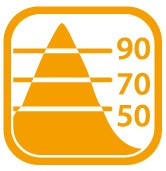
\includegraphics[scale=0.2]{obrazky/INSPIRE_Temata/EL.jpg} &

\includegraphics[scale=0.2]{obrazky/INSPIRE_Temata/SU.jpg} & 
\includegraphics[scale=0.2]{obrazky/INSPIRE_Temata/GE.jpg} & 
\includegraphics[scale=0.2]{obrazky/INSPIRE_Temata/GGS.jpg} & 
\includegraphics[scale=0.2]{obrazky/INSPIRE_Temata/GN.jpg}\\

\includegraphics[scale=0.2]{obrazky/INSPIRE_Temata/HB.jpg} & 
\includegraphics[scale=0.2]{obrazky/INSPIRE_Temata/HH.jpg} &

\includegraphics[scale=0.2]{obrazky/INSPIRE_Temata/HY.jpg} & 
\includegraphics[scale=0.2]{obrazky/INSPIRE_Temata/LC.jpg} & 
\includegraphics[scale=0.2]{obrazky/INSPIRE_Temata/LU.jpg} & 
\includegraphics[scale=0.2]{obrazky/INSPIRE_Temata/MF.jpg}\\

\includegraphics[scale=0.2]{obrazky/INSPIRE_Temata/SD.jpg} & 
\includegraphics[scale=0.2]{obrazky/INSPIRE_Temata/NZ.jpg} &

\includegraphics[scale=0.2]{obrazky/INSPIRE_Temata/SR.jpg} & 
\includegraphics[scale=0.2]{obrazky/INSPIRE_Temata/OI.jpg} & 
\includegraphics[scale=0.2]{obrazky/INSPIRE_Temata/PD.jpg} & 
\includegraphics[scale=0.2]{obrazky/INSPIRE_Temata/PS.jpg}\\
\end{tabular}
\end{center}
\end{center}
\end{frame}

\begin{frame}
\frametitle{Budovy}
\begin{center}

\includegraphics[scale=1]{obrazky/INSPIRE_Temata/BU.jpg}
\end{center}
\end{frame}


\begin{frame}
\frametitle{Aplikační schémata}
\begin{center}
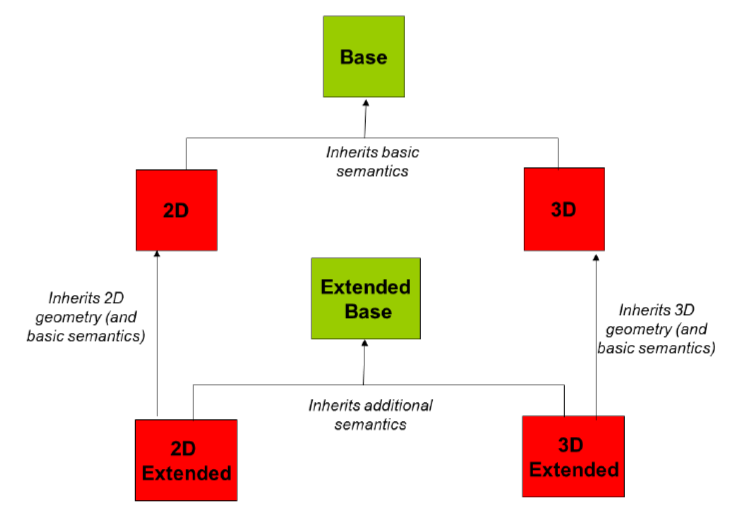
\includegraphics[scale=0.4]{obrazky/app_schema.png}
% celkem šest, dvě abstraktní, čtyři vhodné pro ČR
\end{center}
\end{frame}

\begin{frame}
\frametitle{Schémata XSD}
\begin{itemize}
\item \url{http://www.w3schools.com/schema/}
\end{itemize}
\begin{center}
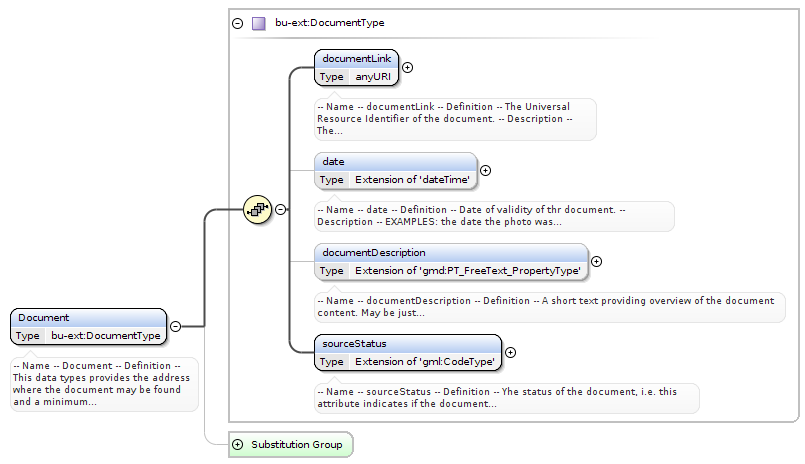
\includegraphics[scale=0.3]{obrazky/XSD.png}
\end{center}
\end{frame}

\begin{frame}
\frametitle{Schémata XSD}
\tiny{
\begin{itemize}
\item \url{http://inspire.ec.europa.eu/schemas/bu-base/3.0/BuildingsBase.xsd}
\item \url{http://inspire.ec.europa.eu/schemas/bu-core2d/3.0/BuildingsCore2D.xsd}
\item \url{http://inspire.ec.europa.eu/schemas/bu-core3d/3.0/BuildingsCore3D.xsd}
\end{itemize}}
\begin{center}

\includegraphics[scale=0.45]{obrazky/missing.jpg}
% pouze tři jsopu zpracované JRC
\end{center}
\end{frame}

\begin{frame}
\frametitle{Rozšiřování aplikačních schémat}
\begin{itemize}
\item Musí vycházet ze stávajících schémat INSPIRE,
\item musí být opatřena dokumentací.
\end{itemize}
\begin{center}
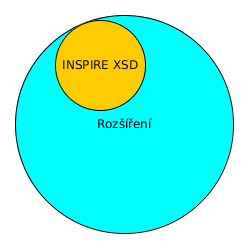
\includegraphics[scale=0.3]{obrazky/extension.png}~
\includegraphics[scale=0.1]{obrazky/rightarrow.png}~
\includegraphics[scale=0.75]{obrazky/data_file.png}
\end{center}
\end{frame}


\begin{frame}
\frametitle{Data INSPIRE}
\begin{itemize}
\item GML 3.2.1 
\end{itemize}
\begin{center}
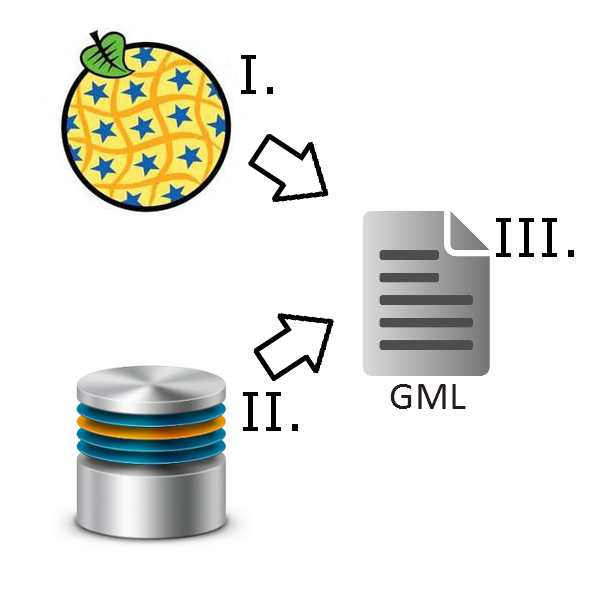
\includegraphics[scale=0.35]{obrazky/data_tvorba.png}
\end{center}
\end{frame}

\begin{frame}
\frametitle{Zdroje dat}
\begin{center}
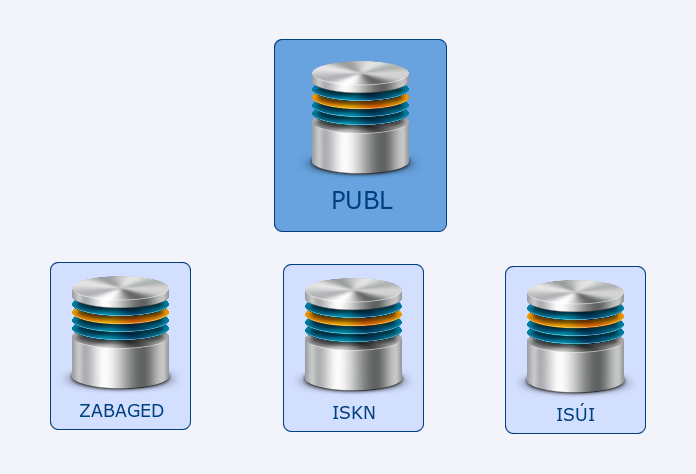
\includegraphics[scale=0.4]{obrazky/data_source.png}
\end{center}
\end{frame}

\begin{frame}
\frametitle{Poskytování a vzhled}
\begin{center}
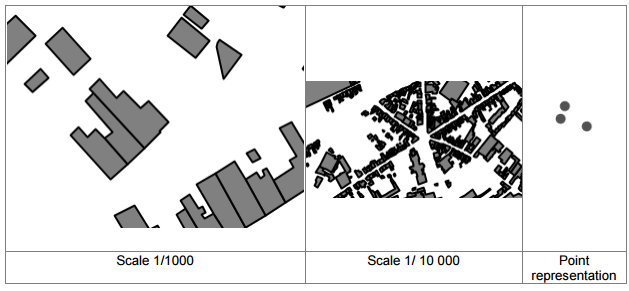
\includegraphics[scale=0.45]{obrazky/portrayal_bu.png}
\end{center}
\end{frame}

\begin{frame}
\frametitle{Poskytování a vzhled}
\begin{center}
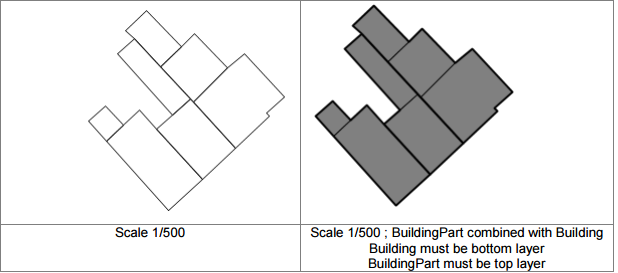
\includegraphics[scale=0.45]{obrazky/portrayal_bp.png}
\end{center}
%více v poslední kapitole
\end{frame}